% astr5400/hw2/hw2.tex
%
% Omkar H. Ramachandran
% omkar.ramachandran@colorado.edu
%
% LaTeX writeup of HW2
%

\documentclass[english]{article}
\usepackage[T1]{fontenc}
\usepackage[latin9]{inputenc}
\usepackage{geometry}
\geometry{verbose,tmargin=1.5in,bmargin=1.5in,lmargin=1.5in,rmargin=1.5in}
\usepackage{babel}
\newcommand{\GeV}{\,{\rm GeV}}
\usepackage{graphicx}
\graphicspath{{./plots/}}
\usepackage{hyperref}
\usepackage{listings}
\usepackage{color}

\lstdefinestyle{custompy}{
  belowcaptionskip=1\baselineskip,
  breaklines=true,
  frame=L,
  xleftmargin=\parindent,
  language=Python,
  showstringspaces=false,
  basicstyle=\footnotesize\ttfamily,
  keywordstyle=\bfseries\color{green},
  commentstyle=\itshape\color{red},
  identifierstyle=\color{black},
  stringstyle=\color{blue},
}


\lstset{escapechar=@,style=custompy}

\begin{document}
\title{ASTR 5400 : Homework 2}
\author{Omkar H. Ramachandran}

\maketitle

\section{Entropy always increases, right? (Spoiler: It does)}
Starting with the second law of thermodynamics we obtain the following 
equation for entropy over time:
\begin{equation}
	\frac{\partial s}{\partial t}+u.\nabla s=-\frac{1}{\rho T}
	\nabla . Q
	\label{eq:entropy}
\end{equation}
We are also given that the system is as follows:
\begin{equation}
	\intop \nabla . QdV = \oint Q.\hat{n}dS = 0
	\label{eq:bc}
\end{equation}

\subsection{Adding 0 on both sides}
Starting with the continuity equation,
\begin{equation}
	\frac{\partial \rho}{\partial t} + \nabla . (\rho u) = 0
	\label{eq:continuity}
\end{equation}
Adding $s\times$(\ref{eq:continuity}) to (\ref{eq:entropy}) (which is valid
since $s(t)>0$ $\forall t$), we obtain the following:
\begin{equation}
	\frac{\partial \rho s}{\partial t}+\nabla.(\rho us)=-\frac{1}{\rho T}
	\nabla .Q 
	\label{eq:morphed}
\end{equation}
The behavior of $s$ as a function of $t$ is outlined in the following 
sections:
\subsection{$Q = -\kappa \nabla T$}
Using some vector gymnastics, we have the following:
$$
	\frac{1}{T}\nabla.(\kappa\nabla T) = 
	\nabla . (\frac{1}{T}\kappa \nabla T) -
	\kappa \nabla T.\nabla\left(\frac{1}{T}\right)
$$
\begin{equation}
	= \nabla . (\frac{1}{T}\kappa \nabla T) + 
	\kappa \frac{\nabla T.\nabla T}{T^{2}}
	= \nabla . (\frac{1}{T}\kappa \nabla T) + 
	\kappa \frac{|\nabla T|^{2}}{T^{2}}
	\label{eq:urghvectors_final}
\end{equation}
Now, we can substitute (\ref{eq:urghvectors_final}) in place of the RHS in
\ref{eq:morphed} to obtain the following:
$$
	\frac{\partial \rho s}{\partial t}+\nabla.(\rho us)=\left(
	\nabla . (\frac{1}{T}\kappa \nabla T) + 
	\kappa \frac{|\nabla T|^{2}}{T^{2}}
	\right)
$$
Rearranging, we have:
\begin{equation}
	\frac{\partial \rho s}{\partial t}=
	-\nabla.\left(\rho us - \frac{1}{T}\kappa \nabla T \right) 
	+\kappa \frac{|\nabla T|^{2}}{T^{2}}
	\label{eq:almost}
\end{equation}
Integrating both sides of (\ref{eq:almost}), we have
$$
	\frac{\partial}{\partial t} \intop \rho sdV=
	-\intop \nabla.\left(\rho us - \frac{1}{T}\kappa \nabla T \right) dV
	+\intop\kappa \frac{|\nabla T|^{2}}{T^{2}}dV
$$
We know from the boundary conditions that $\intop \nabla.QdV = 0$. Thus,
if there's no heat flux out of the system, then the fluid flux 
$\nabla \rho us$ has to compensate, implying that the middle term in the
volume integral vanishes.
Thus, we are left with the following:
\begin{equation}
	\frac{\partial}{\partial t} \intop \rho sdV=
	\intop\kappa \frac{|\nabla T|^{2}}{T^{2}}dV
	\label{eq:done}
\end{equation}
Obviously, $\frac{|\nabla T|^{2}}{T^{2}} \geq 0$ and $\kappa >0$ by 
definition. As a result, that volume integral has to be positive, implying
that the entropy has to monotonically increase with time.

\subsection{$Q = -\kappa \nabla s$}
I'm assuming that $S$ is entropy. I'm also assuming that $\kappa$ refers
specifically to the 'conductivity' -- or it's equivalent, at any rate -- 
of $s$ and not the regular $\kappa$. The units make absolutely no sense 
otherwise. Using the same vector gymnastics as the previous problem, we 
have the following:
$$
	\frac{1}{T}\nabla.(\kappa\nabla s) = 
	\nabla . (\frac{1}{T}\kappa \nabla s) -
	\kappa \nabla s.\nabla\left(\frac{1}{T}\right)
$$
\begin{equation}
	= \nabla . (\frac{1}{T}\kappa \nabla s) + 
	\kappa \frac{\nabla s.\nabla T}{T^{2}}
	\label{eq:urghvectors_final2}
\end{equation}
Now, we can substitute (\ref{eq:urghvectors_final2}) in place of the RHS in
\ref{eq:morphed} to obtain the following:
$$
	\frac{\partial \rho s}{\partial t}+\nabla.(\rho us)=\left(
	\nabla . (\frac{1}{T}\kappa \nabla s) + 
	\kappa \frac{\nabla s\nabla T}{T^{2}}
	\right)
$$
Rearranging, we have:
\begin{equation}
	\frac{\partial \rho s}{\partial t}=
	-\nabla.\left(\rho us - \frac{1}{T}\kappa \nabla s \right) 
	+\kappa \frac{\nabla s\nabla T}{T^{2}}
	\label{eq:almost}
\end{equation}
Integrating both sides of (\ref{eq:almost}), we have
$$
	\frac{\partial}{\partial t} \intop \rho sdV=
	-\intop \nabla.\left(\rho us - \frac{1}{T}\kappa \nabla s \right) dV
	+\intop\kappa \frac{\nabla s \nabla T}{T^{2}}dV
$$
Assuming that $\kappa$ reprasents the equivalent conductivity of $s$, we
can make the same argument as in the previous question. 
If the energy flux of $Q$ - fueled by an entropy gradient - is zero at the 
boundaries, the material flow in the system has to compensate to keep things
physical, thus removing the overall divergence term.
Thus, we are left with the following:
\begin{equation}
	\frac{\partial}{\partial t} \intop \rho sdV=
	\intop\kappa \frac{\nabla s \nabla T}{T^{2}}dV
	\label{eq:done}
\end{equation}
The right hand side, in this case, is guranteed to be greater than zero 
iff $\nabla s >0$ and $\nabla T > 0$ $\forall t>0, {x,y,z}\in V$. Thus,
the function does not have to increase monotonically in time.

\subsection{$Q = - M_{ij} T_{,j}$}
Note: I'm going to use Tensor notation here, simply because the vector
manipulations are obvious when you write them this way.
Defining the same gymnastics in the previous section, we can say the 
following:
\begin{equation}
	\frac{1}{T}\left(M_{ij}T_{,j}\right)_{,j} = 
	\left(\frac{1}{T}M_{ij}T_{,j}\right)_{,j} 
	+\frac{1}{T^{2}}T_{,j}M_{ij}T_{,j}
	\label{eq:tensorsareawesome}
\end{equation}
Now, we can substitute (\ref{eq:tensorsareawesome}) in place of the RHS in
\ref{eq:morphed} to obtain the following:
$$
	\dot{(\rho s)}+(\rho su_{j})_{,j}=\left(\frac{1}{T}M_{ij}T_{,j}\right)_{,j}  
	+\frac{T_{,j}M_{ij}T_{,j}}{T^{2}}
$$
Rearranging, we have:
\begin{equation}
	\dot{(\rho s)}=\left(\rho su_{j}-\frac{1}{T}M_{ij}T_{,j}\right)_{,j}  
	+\frac{T_{,j}M_{ij}T_{,j}}{T^{2}}
	\label{eq:almost}
\end{equation}
Integrating both sides of (\ref{eq:almost}), we have
$$
	\intop \dot{(\rho s)}dV=
	\intop \left(\rho su_{j}-\frac{1}{T}M_{ij}T_{,j}\right)_{,j} dV  
	+ \intop \frac{T_{,j}M_{ij}T_{,j}}{T^{2}} dV
$$
Once again, since $M_{ij}T_{,j}$ reprasents energy, we recycle the argument
made in the previous sections to argue that the overall divergence term is 
zero when integrated over the volume.
Now, $T_{,j}M_{ij}T_{,j}$ is an interesting case. 
If, for instance, 
$M_{ij} = -1 \forall (i,j)$, then entropy does \textbf{not} monotonically
increase.
Interestingly, we sidestepped this particular snag in the previous problem
by assuming that $\kappa > 0$ (which is identical to $M_{ij}=\kappa$). 
However, if we were to assume that $M_{ij}$ is \textbf{positive definite} -
Positive definite matrices have to be symmetric - and not just symmetric, 
then $T_{,j}M_{ij}T_{,j} > 0$, implying that $\rho s$ monotonically
increases.
Was this a typo? 
\subsection{So what does this all mean?}
Basically, to preserve the second law, 'permitted' heat fluxes have to be
such that $\rho s$ monotonically increases with time.
In addition, given that the second law works by asserting that events that
generate through multiple pathways are overwhelmingly more likely than those
with fewer pathways, I wouldn't be surprised if the condition under which
$-\kappa\nabla s$ could work, i.e $\nabla T > 0$ and $\nabla s > 0$ never
really occurs - simply because it is extremely unlikely for it to.
In general, I think we can safely assert that the only possible form of a
heat flux that does not violate the second law in an isolated system is
the one written out in section 1.4, 
$$ Q = -M_{ij}T_{,j} $$
where $M_{ij}$ is - if I'm correct - a positive definite matrix.

\section{Vortices move each other}
The premise is the following: We have two parallel vortex lines of the same
magnitude. The dynamics of this system under the conditions defined in the
subsections below are as follows:
\subsection{Both vortex vectors point in the same direction}
\begin{figure}
	\centering
	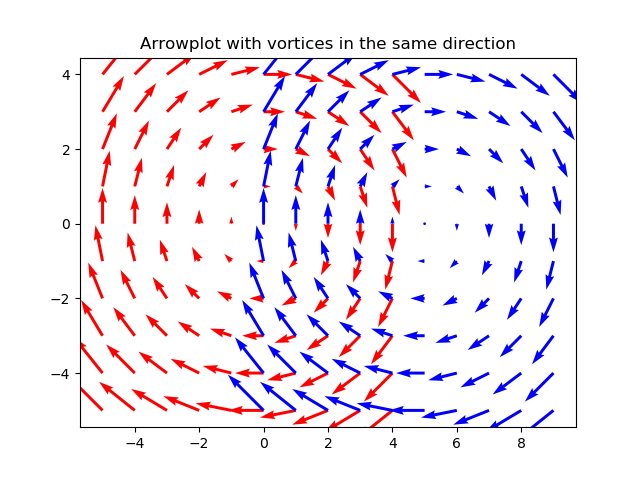
\includegraphics[scale=0.45]{same_direction.png}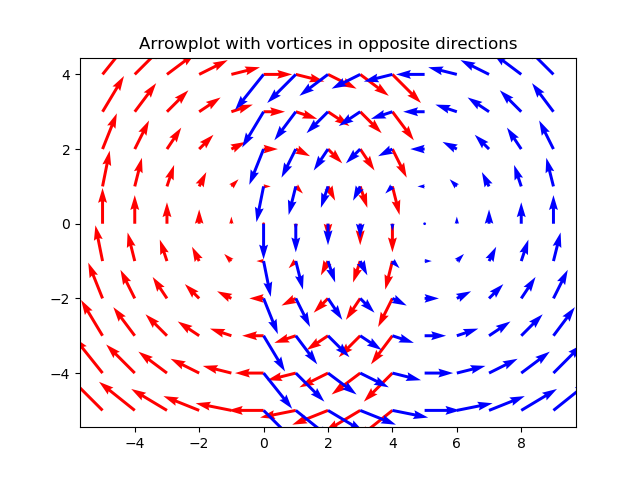
\includegraphics[scale=0.45]{opposite_direction.png}
	\caption{Quiverplot around two parallel vortex vectors pointing (left) 
	in the same direction and (right) in the opposite direction}
	\label{fig:vortices}
\end{figure}
If the two vortex vectors point in the same direction, as in Figure 
\ref{fig:vortices} left, we see that the vector field lines tend to cancel
out in the middle. 
In addition, the further away we are from the center of a vortex, the 
longer the field lines become.
In essence, parallel vortex vectors describe the exact same field, amplified
to reflect the fact the additional vorticity.
Finally, there is no net movement of the center of the vortex, which exists
exactly in between the two lines - where the vector field lines cancel.

\subsection{Both vortex vectors point in different directions}
If the two vortex vectors point in opposite directions, as in Figure 
\ref{fig:vortices} right, we see that the vector field lines add up in the
middle.
This implies that there is a net downward velocity of the system, thus
an observer would see the system drift with a velocity equal to the sum 
of the two vectors directly in the middle.
Of course, there is no net acceleration in the system, thus, one can
transform coordinates to get rid of the net drift and be left with one
vortex of exactly the same magnitude as the one we started with.
This makes perfect sence, of course, since vorticity is guage invariant, 
thus, there is no one unique way of describing a swirling flow.
It is always possible to add in a vortex line in the opposite direction
and transform to coordinates so that the relative velocity between the
observer and the point located between the two vortices is zero.
\end{document}
